\startcontents[localtoc]
\printcontents[localtoc]{}{0}{\subsection*{Contents}\setcounter{tocdepth}{2}}



\phantomsection
\addcontentsline{toc}{section}{Generate sample data}
\subsubsection*{Generate sample data}



Suppose a sine wave of nominal frequency 10 Hz and nominal amplitude 1.5 V is sampled by ADC with
bit resolution of 4 and full range of 1 V. First quantity \texttt{bitres} with number of bits of
resolution of the ADC is prepared and put into input data structure \texttt{DI}.

\begin{lstlisting}
DI = [];
DI.bitres.v = 4;
\end{lstlisting}


Waveform is constructed. Amplitude is selected to overload the ADC.

\begin{lstlisting}
t=[0:1/1e4:1-1/1e4];
Anom = 3.5; fnom = 2; phnom = 0;
wvfrm = Anom*sin(2*pi*fnom*t + phnom);
\end{lstlisting}


Next ADC code values are calculated. It is simulated by quantization and scaling of the sampled
waveform. In real measurement code values can be obtained directly from the ADC. Suppose ADC range
is -2..2.

\begin{lstlisting}
codes = wvfrm;
rmin = -2; rmax = 2;
levels = 2.^DI.bitres.v - 1;
codes(codes<rmin) = rmin;
codes(codes>rmax) = rmax;
codes = round((codes-rmin)./(rmax-rmin).*levels);
\end{lstlisting}


Now lets introduce ADC error. Instead of generating code 2 ADC erroneously generates
code 3 and instead of 11 it generates 10.

\begin{lstlisting}
codes(codes==2) = 3;
codes(codes==11) = 10;
codes = codes + min(codes);
\end{lstlisting}


Create quantity \texttt{codes} and plot a figure with sampled sine wave and codes.

\begin{lstlisting}
DI.codes.v = codes;
figure
hold on
stairs(t, codes);
wvfrm = (wvfrm - rmin)./(rmax-rmin).*levels;
plot(t, wvfrm, '-r');
xlabel('t (s)')
ylabel('Codes / Voltage (scaled)');
legend('Codes generated by ADC','Original waveform scaled to match codes');
hold off
\end{lstlisting}
\begin{center}
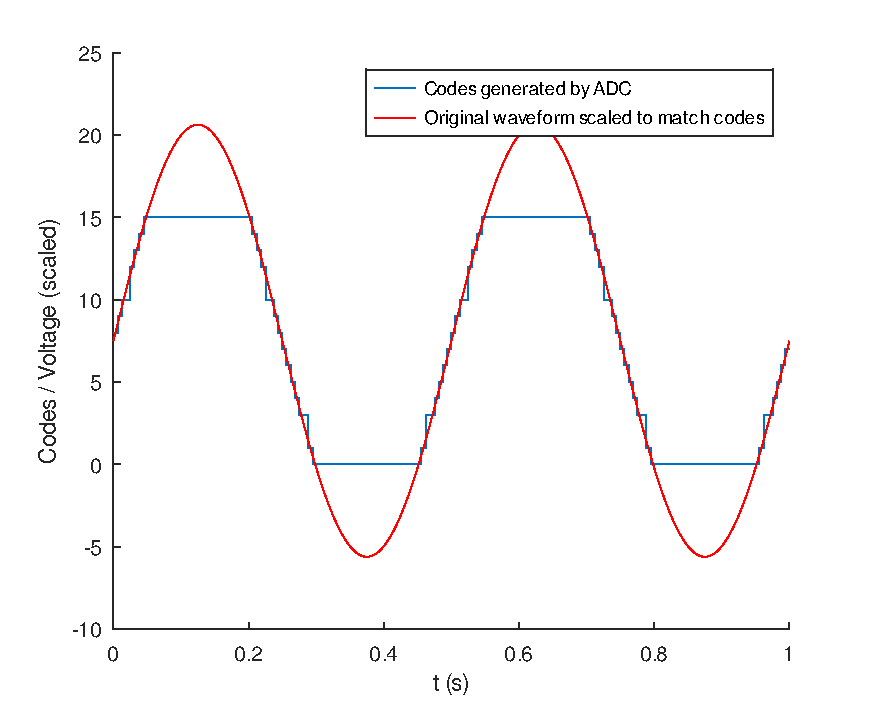
\includegraphics[width=0.7\textwidth]{algs_examples_published/INL-DNL_alg_example-1.pdf}
\end{center}


\phantomsection
\addcontentsline{toc}{section}{Call algorithm}
\subsubsection*{Call algorithm}



Apply INL algorithm to the input data \texttt{DI}.

\begin{lstlisting}
DO = qwtb('INL-DNL', DI);
\end{lstlisting}
\begin{lstlisting}[language={},xleftmargin=5pt,frame=none]
QWTB: no uncertainty calculation
warning: Invalid UTF-8 byte sequences have been replaced.
warning: called from
    ProcessHistogramTest at line 52 column 3
    alg_wrapper at line 35 column 5
    qwtb>check_and_run_alg at line 377 column 17
    qwtb at line 114 column 47
    publish>eval_code_helper at line 1079 column 8
    publish>eval_code at line 995 column 30
    publish at line 402 column 9
    all_algs_examples2tex at line 51 column 5
 
warning: Invalid UTF-8 byte sequences have been replaced.
warning: called from
    ProcessHistogramTest at line 273 column 14
    alg_wrapper at line 35 column 5
    qwtb>check_and_run_alg at line 377 column 17
    qwtb at line 114 column 47
    publish>eval_code_helper at line 1079 column 8
    publish>eval_code at line 995 column 30
    publish at line 402 column 9
    all_algs_examples2tex at line 51 column 5
 

\end{lstlisting}


Plot results of integral non-linearity. One can clearly observe defects on codes 3 and
11.

\begin{lstlisting}
figure
plot(DO.INL.v, '-x');
xlabel('Transition levels')
ylabel('INL (k)')
\end{lstlisting}
\begin{center}
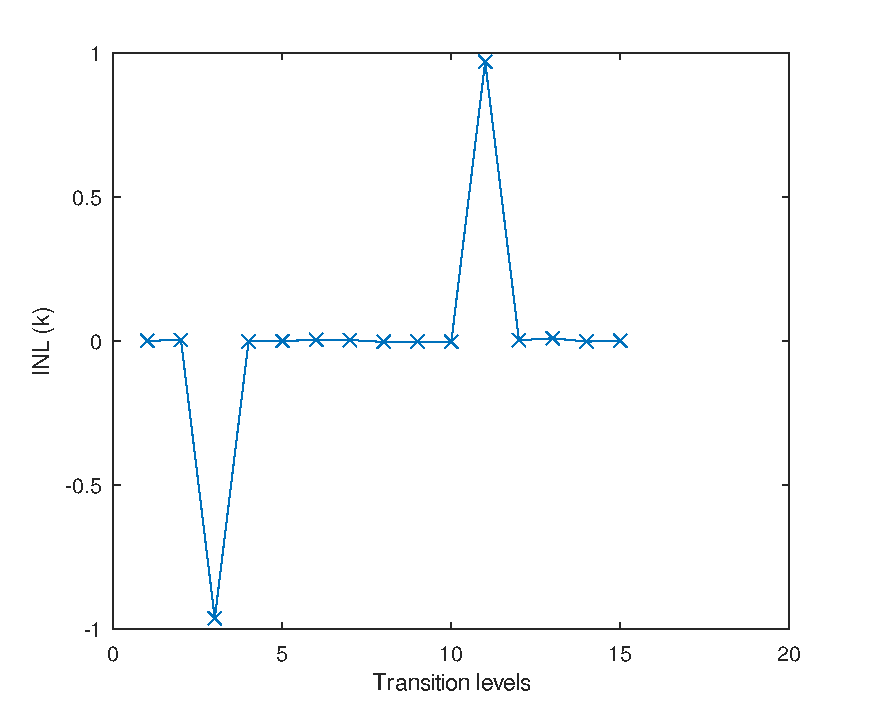
\includegraphics[width=0.7\textwidth]{algs_examples_published/INL-DNL_alg_example-2.pdf}
\end{center}


Plot results of differential non-linearity. One can clearly observe defects on transitions 2-3 and
10-11.

\begin{lstlisting}
figure
plot(DO.DNL.v, '-x');
xlabel('Code bins')
ylabel('DNL (k)')
\end{lstlisting}
\begin{center}
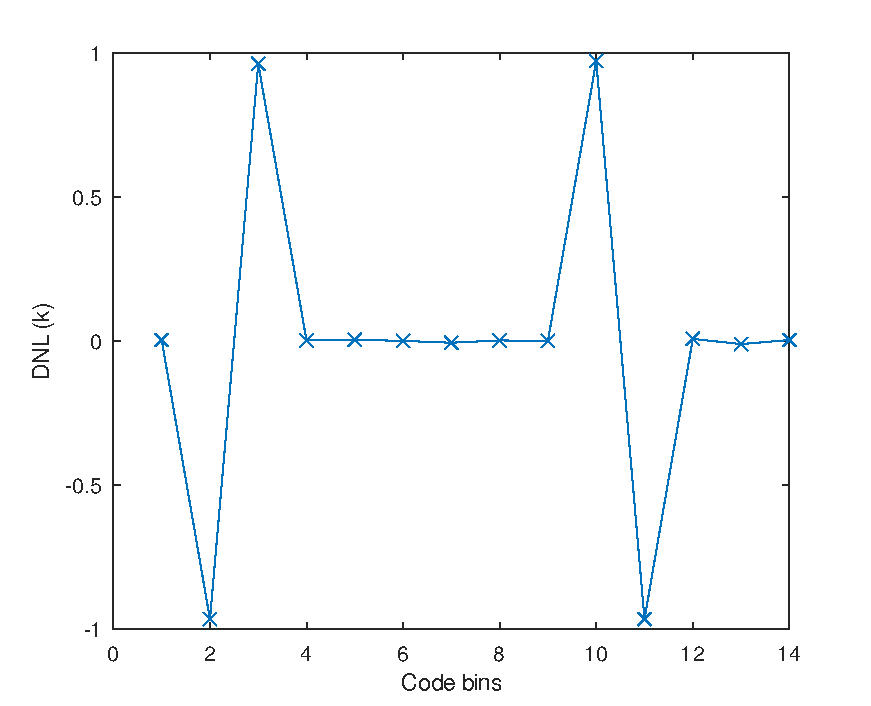
\includegraphics[width=0.7\textwidth]{algs_examples_published/INL-DNL_alg_example-3.pdf}
\end{center}


\stopcontents[localtoc]
